After summarizing the data, two types of graphs - a scatter plot and a double bar graph were plotted to better understand how each feature affected the result.  \\

The dataset was divided into two classes - \textbf{legitimate} and \textbf{phishing} to easily inspect the data.
One of the main features of the dataset was the length of URL and the length of hostname. Phishing websites are normally said to have long URLs to hide certain parts of the URL. A scatter plot was drawn to see the  visibility of this feature  in the dataset. \\

Double bar graphs were also plotted to compare how the remaining features varied for both the classes. 


\begin{Figure}
	
 \centering
 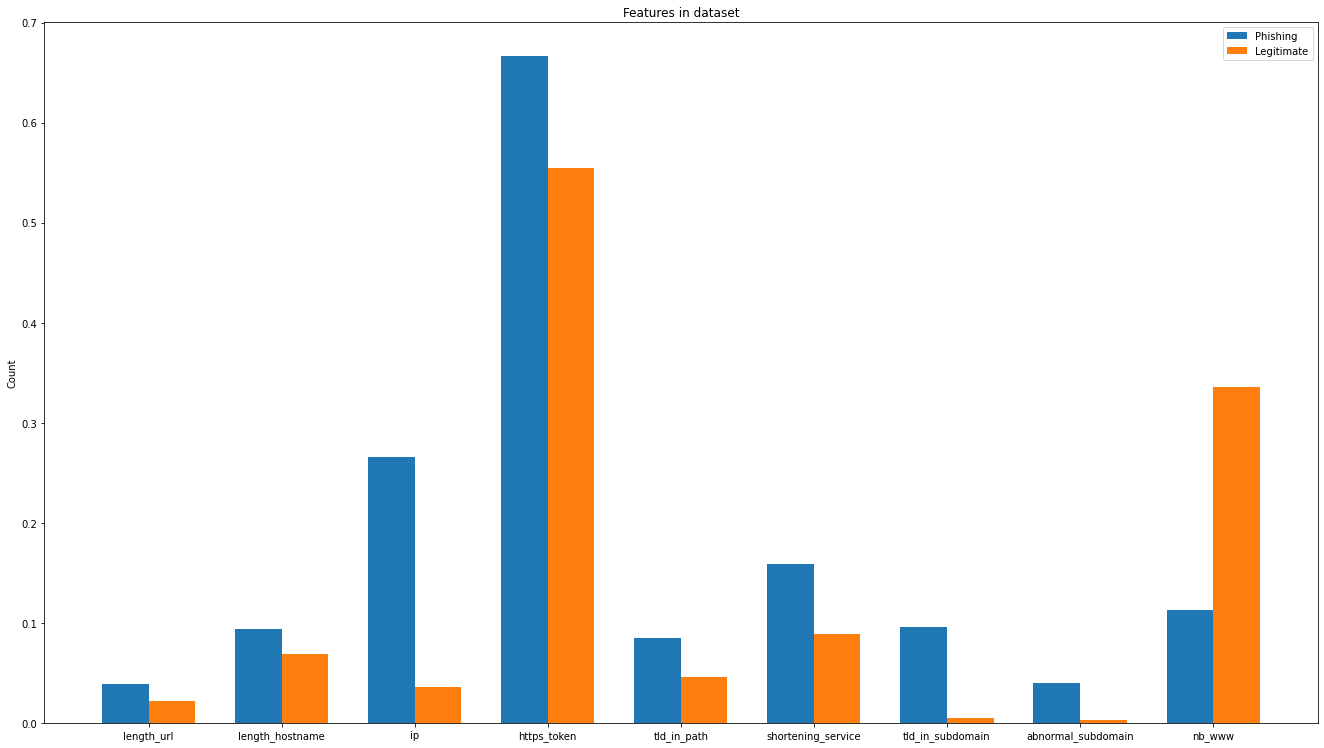
\includegraphics[width=\linewidth]{bar_1.png}
 
 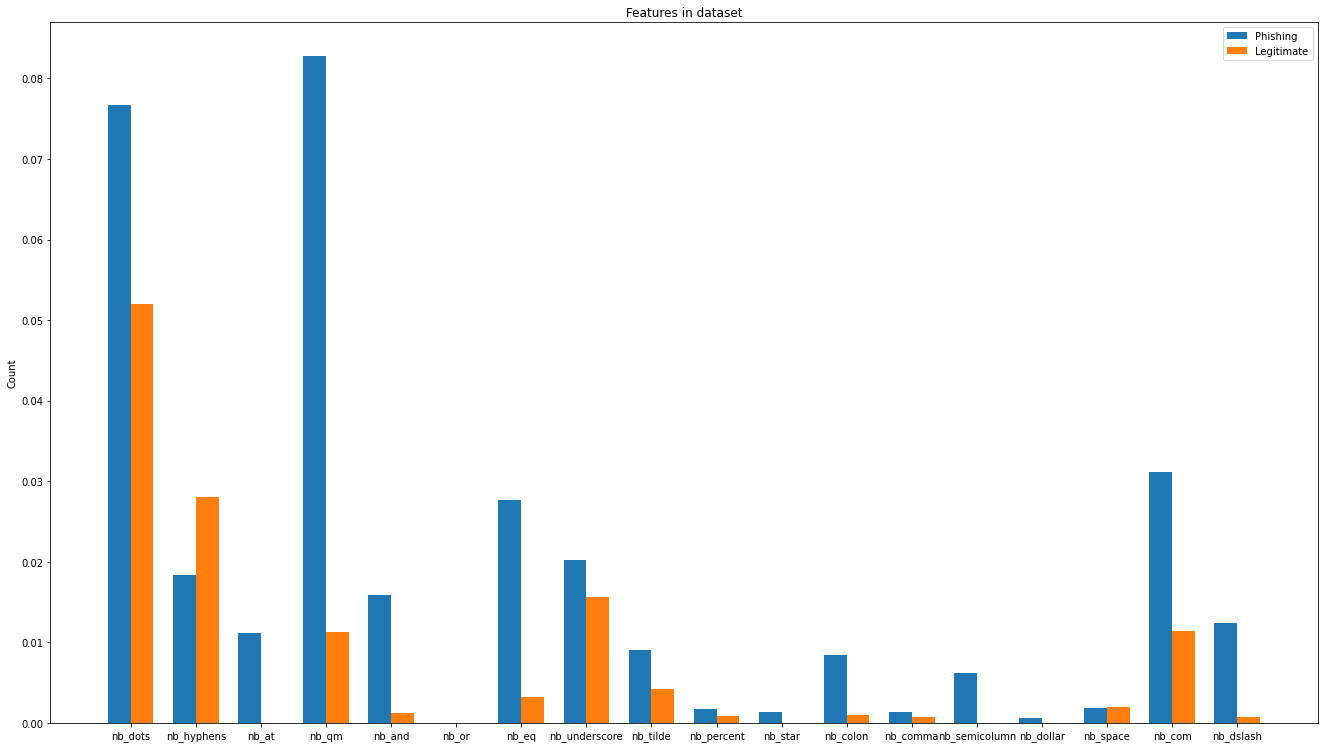
\includegraphics[width=\linewidth]{bar_2.png}
 \captionof{figure}{Double bar graphs depecting how features vary in legitimate and phishing URLs.}
\end{Figure}